\lstset{
style=python,
morekeywords={[2]
factorial,
fibonacci,
hanoi,
palindrome,
exponentiation,
multiplication,
code
}
}

\section{Silnia}\label{sec:silnia}
\begin{frame}{Wzory}
    \begin{definition}
        \[ n! = \prod\limits_{k = 1}^{n}k \qquad \text{, for } n \geq 1 \]
        \[ 0! = 1 \]
    \end{definition}
    \begin{definition}[recursion]
        \[ n! =
        \begin{cases}
            1 & \text{, for } n = 0 \\
            n \cdot (n - 1)! & \text{, for } n \geq 1
        \end{cases}
        \]
    \end{definition}
\end{frame}
\begin{frame}[fragile]{Kod w Pythonie}
    \lstinputlisting{code/factorial.py}
\end{frame}
\begin{frame}{Stos wywołań funkcji}
    \centering
    starting with 5\\
    starting with 4\\
    starting with 3\\
    starting with 2\\
    starting with 1\\
    starting with 0\\
    ending with 0\\
    ending with 1\\
    ending with 2\\
    ending with 3\\
    ending with 4\\
    ending with 5\\
\end{frame}
%%%%%%%%%%%%%%%%
\section{Ciąg Fibonacciego}\label{sec:ciągFibonacciego}
\begin{frame}{Króliki Fibonacciego}
    \centering
    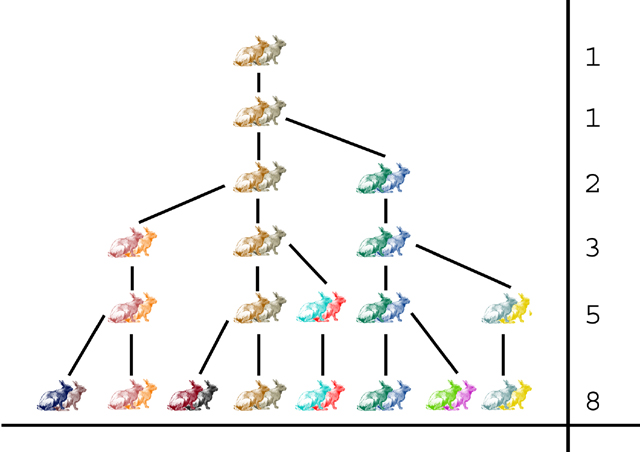
\includegraphics[height=0.8\textheight]{graphics/recursion/fibonacci_rabbits.jpg}
\end{frame}
\begin{frame}[fragile]{Kod w Pythonie}
    \lstinputlisting{code/fibonacci.py}
\end{frame}
%%%%%%%%%%%%%%%%
\begin{frame}{Stos i drzewo wywołań funkcji}
    \centering
    \begin{columns}
        \begin{column}{0.25\textwidth}
            \textcolor{black}{starting with 5}\\
            \textcolor{black}{starting with 4}\\
            \textcolor{black}{starting with 3}\\
            \textcolor{black}{starting with 2}\\
            \textcolor{black}{starting with 1}\\
            \textcolor{black}{ending with 1}\\
            \textcolor{black}{starting with 0}\\
            \textcolor{black}{ending with 0}\\
            \textcolor{black}{ending with 2}\\
            \textcolor{black}{starting with 1}\\
            \textcolor{black}{ending with 1}\\
            \textcolor{black}{ending with 3}\\
            \textcolor{black}{starting with 2}\\
            \textcolor{black}{starting with 1}\\
            \textcolor{black}{ending with 1}\\
        \end{column}
        \begin{column}{0.25\textwidth}
            \textcolor{black}{starting with 0}\\
            \textcolor{black}{ending with 0}\\
            \textcolor{black}{ending with 2}\\
            \textcolor{black}{ending with 4}\\
            \textcolor{black}{starting with 3}\\
            \textcolor{black}{starting with 2}\\
            \textcolor{black}{starting with 1}\\
            \textcolor{black}{ending with 1}\\
            \textcolor{black}{starting with 0}\\
            \textcolor{black}{ending with 0}\\
            \textcolor{black}{ending with 2}\\
            \textcolor{black}{starting with 1}\\
            \textcolor{black}{ending with 1}\\
            \textcolor{black}{ending with 3}\\
            \textcolor{black}{ending with 5}\\
        \end{column}
        \begin{column}{0.5\textwidth}
            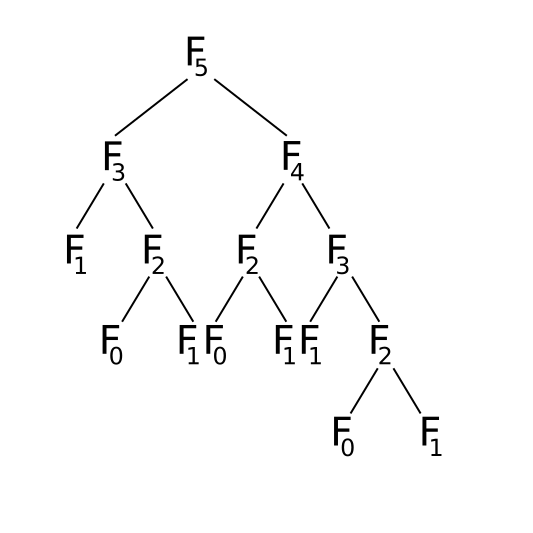
\includegraphics[width=\textwidth]{graphics/recursion/fibonacci_black.png}
        \end{column}
    \end{columns}
\end{frame}
%%%%%%%%%%%%%%%%
\begin{frame}{Stos i drzewo wywołań funkcji}
    \centering
    \begin{columns}
        \begin{column}{0.25\textwidth}
            \textcolor{black}{starting with 5}\\
            \textcolor{black}{starting with 4}\\
            \textcolor{black}{starting with 3}\\
            \textcolor{blue}{starting with 2}\\
            \textcolor{orange}{starting with 1}\\
            \textcolor{orange}{ending with 1}\\
            \textcolor{red}{starting with 0}\\
            \textcolor{red}{ending with 0}\\
            \textcolor{blue}{ending with 2}\\
            \textcolor{black}{starting with 1}\\
            \textcolor{black}{ending with 1}\\
            \textcolor{black}{ending with 3}\\
            \textcolor{blue}{starting with 2}\\
            \textcolor{orange}{starting with 1}\\
            \textcolor{orange}{ending with 1}\\
        \end{column}
        \begin{column}{0.25\textwidth}
            \textcolor{red}{starting with 0}\\
            \textcolor{red}{ending with 0}\\
            \textcolor{blue}{ending with 2}\\
            \textcolor{black}{ending with 4}\\
            \textcolor{black}{starting with 3}\\
            \textcolor{blue}{starting with 2}\\
            \textcolor{orange}{starting with 1}\\
            \textcolor{orange}{ending with 1}\\
            \textcolor{red}{starting with 0}\\
            \textcolor{red}{ending with 0}\\
            \textcolor{blue}{ending with 2}\\
            \textcolor{black}{starting with 1}\\
            \textcolor{black}{ending with 1}\\
            \textcolor{black}{ending with 3}\\
            \textcolor{black}{ending with 5}\\
        \end{column}
        \begin{column}{0.5\textwidth}
            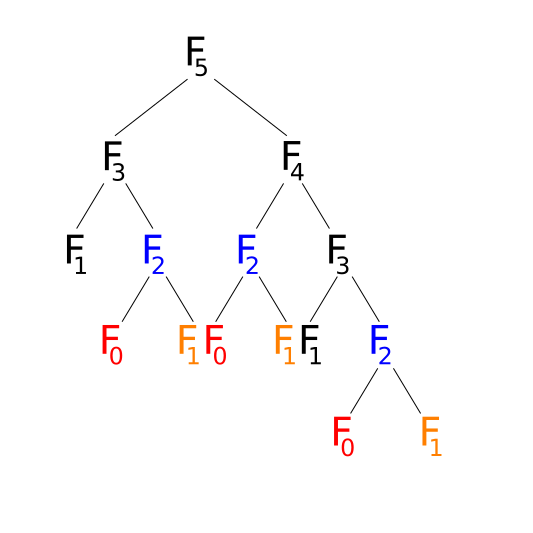
\includegraphics[width=\textwidth]{graphics/recursion/fibonacci_F3.png}
        \end{column}
    \end{columns}
\end{frame}
%%%%%%%%%%%%%%%%
\begin{frame}{Stos i drzewo wywołań funkcji}
    \centering
    \begin{columns}
        \begin{column}{0.25\textwidth}
            \textcolor{black}{starting with 5}\\
            \textcolor{black}{starting with 4}\\
            \textcolor{magenta}{starting with 3}\\
            \textcolor{blue}{starting with 2}\\
            \textcolor{orange}{starting with 1}\\
            \textcolor{orange}{ending with 1}\\
            \textcolor{red}{starting with 0}\\
            \textcolor{red}{ending with 0}\\
            \textcolor{blue}{ending with 2}\\
            \textcolor{green}{starting with 1}\\
            \textcolor{green}{ending with 1}\\
            \textcolor{magenta}{ending with 3}\\
            \textcolor{black}{starting with 2}\\
            \textcolor{black}{starting with 1}\\
            \textcolor{black}{ending with 1}\\
        \end{column}
        \begin{column}{0.25\textwidth}
            \textcolor{black}{starting with 0}\\
            \textcolor{black}{ending with 0}\\
            \textcolor{black}{ending with 2}\\
            \textcolor{black}{ending with 4}\\
            \textcolor{magenta}{starting with 3}\\
            \textcolor{blue}{starting with 2}\\
            \textcolor{orange}{starting with 1}\\
            \textcolor{orange}{ending with 1}\\
            \textcolor{red}{starting with 0}\\
            \textcolor{red}{ending with 0}\\
            \textcolor{blue}{ending with 2}\\
            \textcolor{green}{starting with 1}\\
            \textcolor{green}{ending with 1}\\
            \textcolor{magenta}{ending with 3}\\
            \textcolor{black}{ending with 5}\\
        \end{column}
        \begin{column}{0.5\textwidth}
            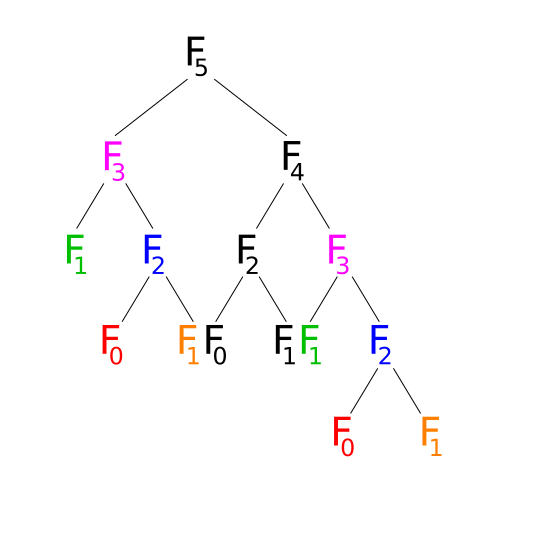
\includegraphics[width=\textwidth]{graphics/recursion/fibonacci_F4.png}
        \end{column}
    \end{columns}
\end{frame}
\begin{frame}{Skierowany graf acykliczny}
    \centering
    \begin{columns}
        \begin{column}{0.5\textwidth}
            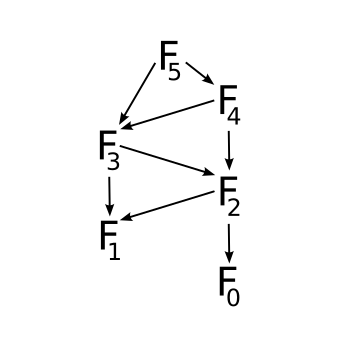
\includegraphics[width=1.2\textwidth,height=0.7\textheight]{graphics/recursion/fibonacci_dag.png}
        \end{column}
        \begin{column}{0.5\textwidth}
            Pewnie zauważyliście, że wiele z funkcji liczy się wielokrotnie dla tych samych danych, co powoduje znaczące wydłużenie działania programu. \\
            Rozwiązaniem tego problemu jest programowanie dynamiczne, prowadzące do drzewa wywołań w formie DAGu, czyli skierowanego grafu acyklicznego.
        \end{column}
    \end{columns}
\end{frame}
%%%%%%%%%%%%%%%%

\section{Wieża Hanoi}\label{sec:wieżaHanoi}
\begin{frame}{Legenda}
    \begin{quote}
        \quad Pod kopułą świątyni Brahmy w Benares znajduje się tablica z brązu, na której umieszczone są trzy diamentowe słupki. Na jednym z tych słupków Bóg umieścił sześćdziesiąt cztery krążki z czystego złota. W ten sposób powstała wieża z Brahmy. \\
        \quad Dniem i nocą mnisi z pobliskiego klasztoru przekładają krążki z jednego diamentowego słupka na drugi zgodnie z wyznaczonymi regułami. \\
        \quad Kiedy wszystkie sześćdziesiąt cztery krążki zostaną przeniesione ze słupka, na którym umieścił je Bóg, na inny słupek, to wszystko - słupki , wieża, świątynia i mnisi - zamieni się w pył i cały świat ulegnie zniszczeniu.
    \end{quote}
\end{frame}
\begin{frame}{Działanie}
    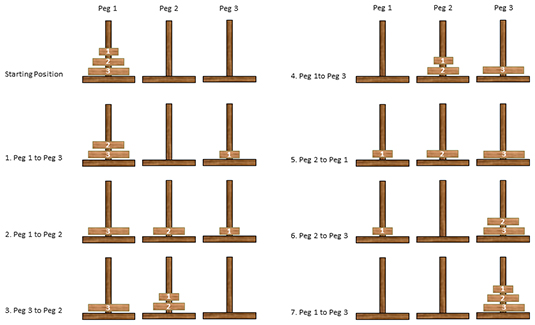
\includegraphics[width=\textwidth,height=0.8\textheight]{graphics/recursion/hanoi_tower.jpg}
\end{frame}
\begin{frame}[fragile]{Kod w Pythonie}
    \lstinputlisting{code/hanoi.py}
\end{frame}
\begin{frame}{Wynik działania kodu}
    \centering
    Moving 1th disk from A to C using B as assistant\\
    Moving 2th disk from A to B using C as assistant\\
    Moving 1th disk from C to B using A as assistant\\
    Moving 3th disk from A to C using B as assistant\\
    Moving 1th disk from B to A using C as assistant\\
    Moving 2th disk from B to C using A as assistant\\
    Moving 1th disk from A to C using B as assistant\\
    Moving 4th disk from A to B using C as assistant\\
    Moving 1th disk from C to B using A as assistant\\
    Moving 2th disk from C to A using B as assistant\\
    Moving 1th disk from B to A using C as assistant\\
    Moving 3th disk from C to B using A as assistant\\
    Moving 1th disk from A to C using B as assistant\\
    Moving 2th disk from A to B using C as assistant\\
    Moving 1th disk from C to B using A as assistant\\
\end{frame}
\begin{frame}{Wielkość problemu}
    Dla każdej kolejnej wartości problem jest dwa razy większy - liczy się dwa razy dłużej. \\
    h(n) to ilość koniecznych do wykonania przemieszczeń pojedyńczego dysku dla n-dużego problemu. \\
    \[ h(1) = 1 \]
    \[ h(n) = h(n-1) + 1 + h(n-1) \]
    \[ h(n) = 2 \cdot h(n-1) + 1 \]
    \[ H(n) = h(n) + 1 = 2(h(n-1) + 1) \]
    \[ H(n) = 2 \cdot H(n-1) \]
    \[ H(1) = 2 \]
    \[ H(n) = 2^n \]
    \[ h(n) = 2^n - 1 \]
\end{frame}
\begin{frame}{Wielkość problemu}
    Problem rośnie wykładniczo, podobnie jak w legendzie o wynalezieniu szachów. Wzór na liczbę ziarenek (ciąg geometryczny o $a_1=1, q=2$) na n-tym polu wynosi $r(n) = 2^{n-1}$. \\
    Wzór na sumę wszystkich ziarenek (suma pierwszych wyrazów ciągu) do n-tego pola włącznie wynosi:
    \[ S_r(n) = a_1 \cdot \frac{1-q^n}{1-q} = 1 \cdot \frac{1-2^n}{1-2} = 2^n - 1 \]
    \centering
    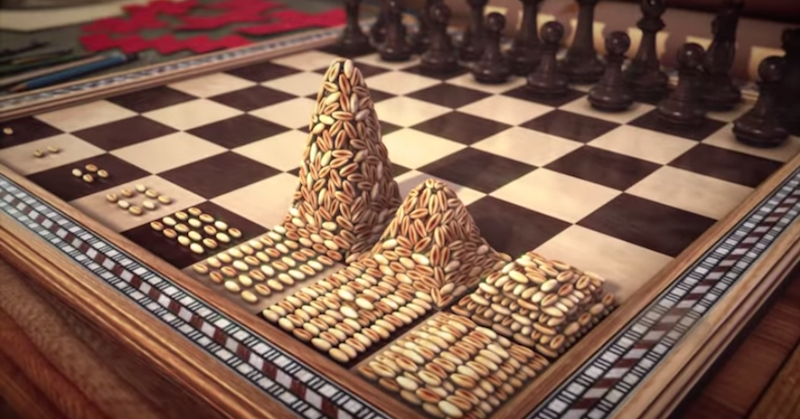
\includegraphics[height=0.35\textheight]{graphics/recursion/chessboard1.png}
\end{frame}
\begin{frame}{Wielkość problemu}
    \centering
    \begin{columns}
        \begin{column}{0.5\textwidth}
            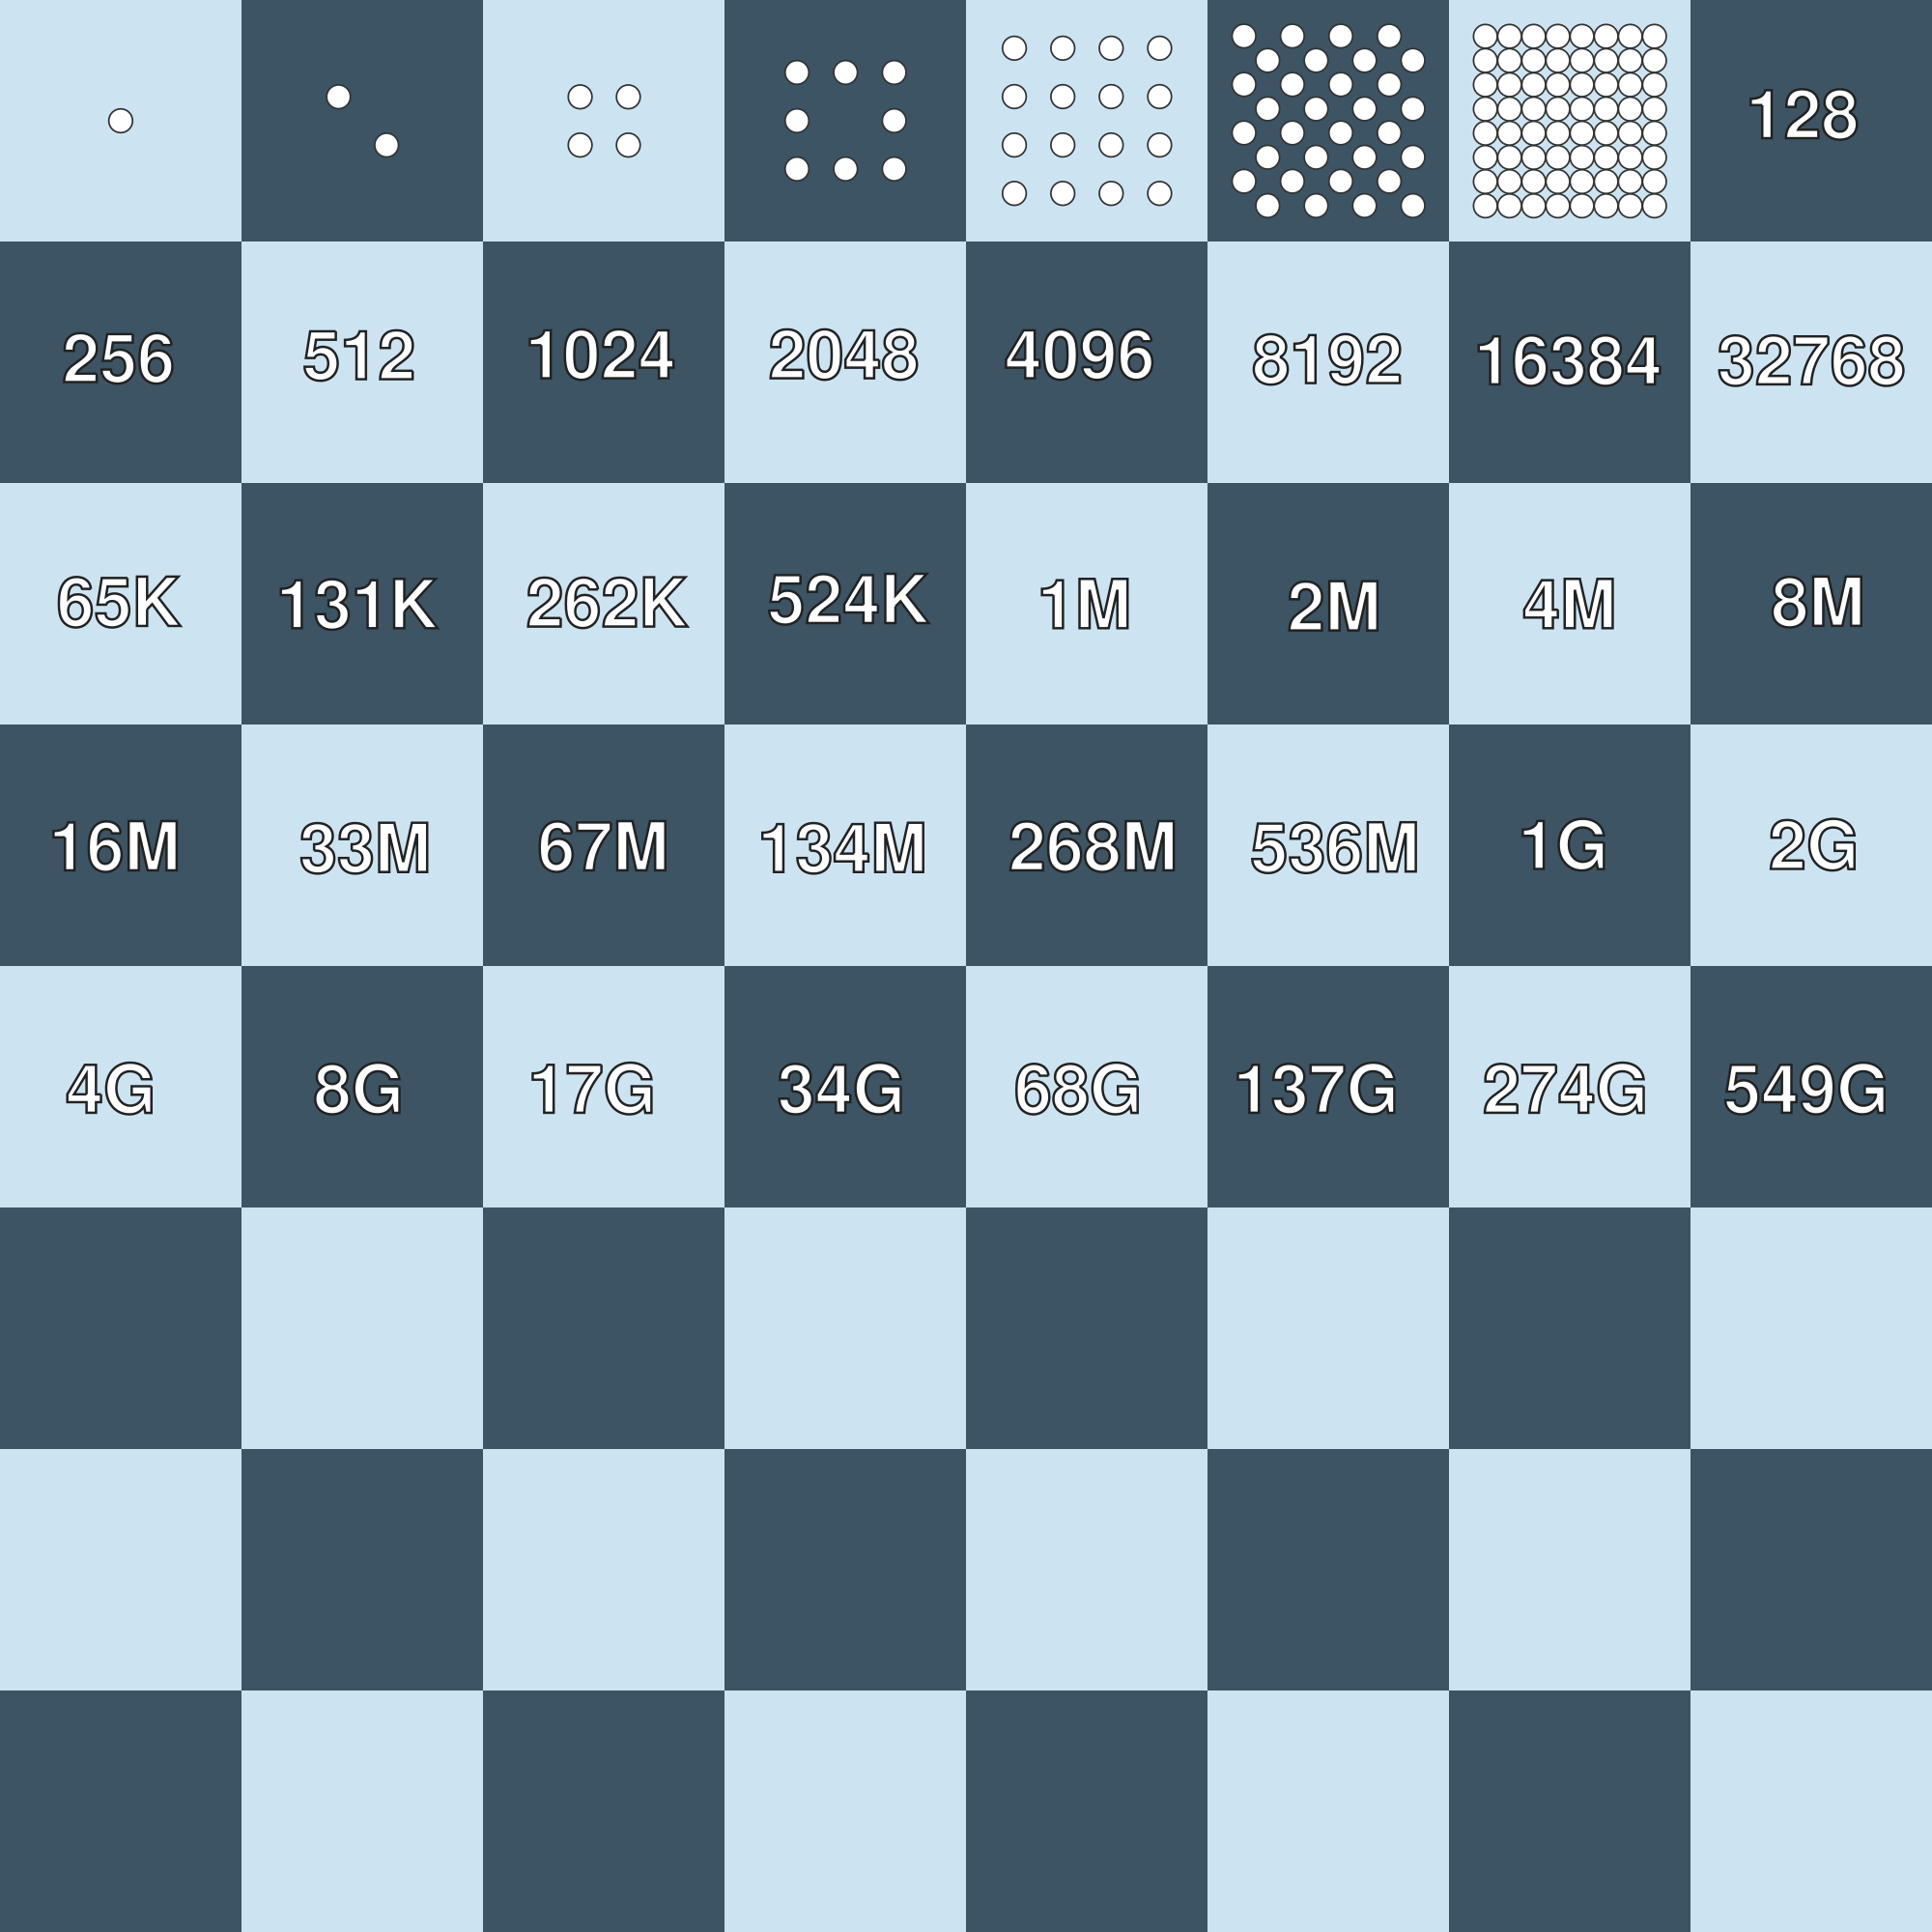
\includegraphics[height=0.7\textheight]{graphics/recursion/chessboard2.png}
        \end{column}
        \begin{column}{0.5\textwidth}
            W przypadku szachownicy mamy łącznie na wszystkich 64 polach $S_r(64)$ ziarenek ryżu. \\
            W przypadku wieży hanoi dla 64 dysków mamy $h(64)$ koniecznych przesunięć.
            \[ S_r(64) = 2^{64} - 1 = h(64) \]
            \[ 2^{64} - 1 = 18.446744 \cdot 10^{18} \]
        \end{column}
    \end{columns}
\end{frame}
%%%%%%%%%%%%%%%%
\section{Palindromy}\label{sec:palindromy}
\begin{frame}[fragile]{Kod w Pythonie}
    \lstinputlisting{code/palindrome.py}
\end{frame}
%%%%%%%%%%%%%%%%
\section{Potęgowanie}\label{sec:potęgowanie}
\begin{frame}{Wzory}
    \begin{definition}[recursion]
        \[ i^j =
        \begin{cases}
            1 & \text{, for } j = 0 \land i \neq 0 \\
            i \cdot i^{(j-1)} & \text{, for } j \geq 1 \\
            \Big( \frac{1}{i} \Big) ^{-j} & \text{, for } j \leq -1
        \end{cases}
        \]
    \end{definition}
\end{frame}
\begin{frame}[fragile,allowframebreaks]{Kod w Pythonie}
    \lstinputlisting{code/exponentiation.py}
    \lstinputlisting{code/exponentiation_test.py}
\end{frame}
%%%%%%%%%%%%%%%%
\section{Mnożenie}\label{sec:mnożenie}
\begin{frame}[allowframebreaks]{Wzory}
    \begin{definition}[recursion 1]
        \[ i \cdot j =
        \begin{cases}
            -i + (i \cdot (j+1)) & \text{, for } j \leq -1 \\
            0 & \text{, for } j = 0 \\
            1 & \text{, for } j = 1 \\
            i + (i \cdot (j-1)) & \text{, for } j \geq 2
        \end{cases}
        \]
    \end{definition}
    \begin{definition}[recursion 2]
        \[ i \cdot j =
        \begin{cases}
            -(i \cdot (-j)) & \text{, for } j \leq -1 \\
            0 & \text{, for } j = 0 \\
            1 & \text{, for } j = 1 \\
            i + (i \cdot (j-1)) & \text{, for } j \geq 2
        \end{cases}
        \]
    \end{definition}
    \begin{definition}[recursion 3.1]
        \[ i \cdot j =
        \begin{cases}
            0 & \text{, for } j = 0 \lor i = 0 \\
            -(i \cdot (-j)) & \text{, for } j < 0 \\
            -((-i) \cdot j) & \text{, for } i < 0 \\
            (j \cdot i) & \text{, for } i < j \\
            (i * j) & \text{, otherwise}
        \end{cases}
        \]
    \end{definition}
    \begin{definition}[recursion 3.2]
        \[ i * j =
        \begin{cases}
            i & \text{, for } j = 1 \\
            (i * (j-1)) & \text{, otherwise}
        \end{cases}
        \]
    \end{definition}
\end{frame}
\begin{frame}[fragile,allowframebreaks]{Kod w Pythonie}
    \lstinputlisting{code/multiplication_1.py}
    \lstinputlisting{code/multiplication_2.py}
    \lstinputlisting{code/multiplication_3.py}
\end{frame}
\begin{frame}[fragile,allowframebreaks]{Trochę o złożoności i optymalizacji}
    Oznaczmy czasy:
    \begin{itemize}
        \item przez E czas porównania dwóch wartości. \\
        \item przez C czas operacji potrzebnych do pojedyńczego wejścia do funkcji i wyjścia z niej, nie wliczając czasu operacji wewnątrz. \\
        \item przez O czas podstawowej operacji matematycznej, takiej jak dodanie dwóch wartości, zamiana liczby na przeciwną, itp
    \end{itemize}
    Ile i jakiego typu operacji wystąpi w mnożeniu $(-2) \cdot 20$? \\
    Zastanówmy się: \\
    1 przebieg: 1 C, 3 E, 2 O. \\
    Wiecie czemu? \\
    Wszystkie przebiegi wyniosą 30 C, 10 E, 18 O. \\
    Tutaj wystarczyło pomnożyć, jednak dla np.: $(-2) \cdot (-5)$ wyjdzie 7 C, 6 E, 10 O, przy pierwszym przebiegu 1 E, 1 C, 3 O. \\
    Tutaj mnożenie się nie sprawdzi. \\
    Zastanówmy się skąd dokładnie biorą się te liczby. \\
    Pomoże nam w tym kod zedytowany tak, by zliczał ile razy musiał wykonać odpowiednią operację.
    \lstinputlisting{code/multiplication_1b.py}
    Czy gdy zamienimy kolejnością instrukcje otrzymamy inne wyniki? \\
    Co z pozostałymi funkcjami mnożącymi które napisaliśmy? \\
    Sprawdźcie to dla różnych funkcji i danych wejściowych.
\end{frame}
%%%%%%%%%%%%%%%%
\section{Inne problemy rekurencyjne}\label{sec:inneProblemyRekurencyjne}
\begin{frame}{Sortowanie przez scalanie}
    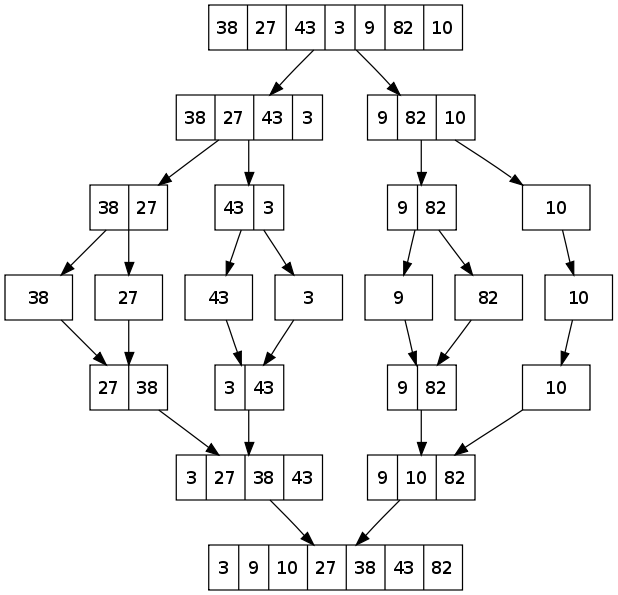
\includegraphics[width=\textwidth,height=0.8\textheight]{graphics/recursion/mergesort.png}
\end{frame}
\begin{frame}{Sortowanie szybkie}
    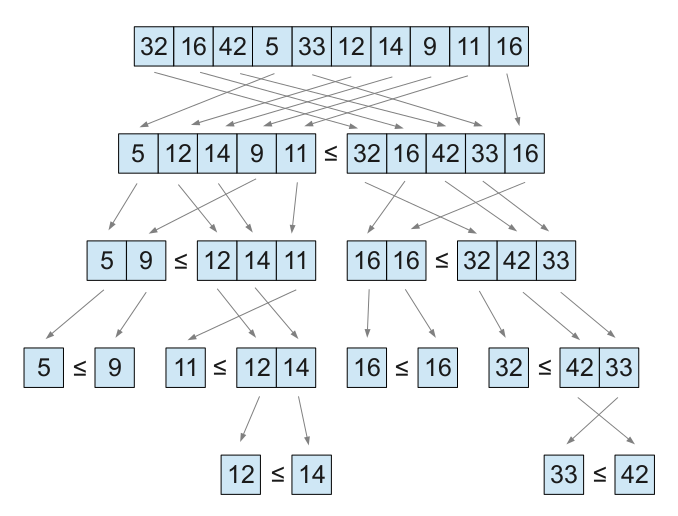
\includegraphics[width=\textwidth,height=0.8\textheight]{graphics/recursion/quicksort.png}
\end{frame}
\begin{frame}{Problem skoczka}
    \centering
    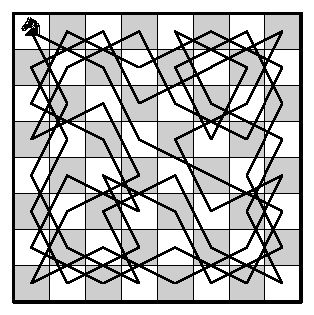
\includegraphics[height=0.8\textheight]{graphics/recursion/knight_tour.jpg}
\end{frame}
\begin{frame}[allowframebreaks]{Zadania i problemy}
    \begin{enumerate}
        \item Napisz algorytm iteracyjnego obliczania silnii i porównaj czasy wykonania z algorytmem rekurencyjnym. Zastanów się, dlaczego silnia nazywana jest antyprzykładem rekurencji? \\
        \item Oblicz ilość wywołań funkcji obliczającej n-ty wyraz ciągu fibonacciego dla n-dużego problemu. Czy można go uprościć do jakiegoś wzoru jawnego (nierekurencyjnego)? Poczytaj o funkcjach tworzących i wzorze Bineta. \\
        \item Pobaw się klasą Tower dla n = 64 tak jak w legendzie. Zostaw tower.plot_loop_steps(0.1) na noc i sprawdź do którego krążka doszedł program nad ranem. \\
        \item Napisz program do testowania palindromów który mieści się w jednej linijce i ma \textcolor{green}{\checkmark} w PyCharmie, tzn nie wywołuje errorów ani warningów, a ctrl+l go nie poprawia. Porównaj czas i poprawność jego działania z algorytmem rekurencyjnym. Program który ja napisałem miał 107 znaków - spróbuj napisać krótszy! \\
        \item Przeprowadź analizę koniecznych operacji dla pozostałych algorytmów mnożenia rekurencyjnego. Dodaj w kodzie fragmenty odpowiedzialne za policzenie operacji i przetestuj wszystkie algorytmy dla różnych danych wejściowych. Zastanów się, jakie są optymistyczne i pesymistyczne przypadki wywołania różnych algorytmów? \\
        \item Zaimplementuj bardziej optymalną twoim zdaniem wersję potęgowania rekurencyjnego. Przeprowadź jej analizę i porównaj z algorytmem z tej prezentacji. \\
        \item Zaimplementuj jedno z sortowań rekurencyjnych. \\
        \item Zastanów się dla jakiego rozmiaru problemu skoczka nie ma rozwiązania, nawet otwartego. Spróbuj zaimplementować algoytm rozwiązujący problem. \\
    \end{enumerate}
\end{frame}